% Compile from the manuscript main/ directory with graphicx and booktabs.
\begin{figure}[tbp]
  \centering
  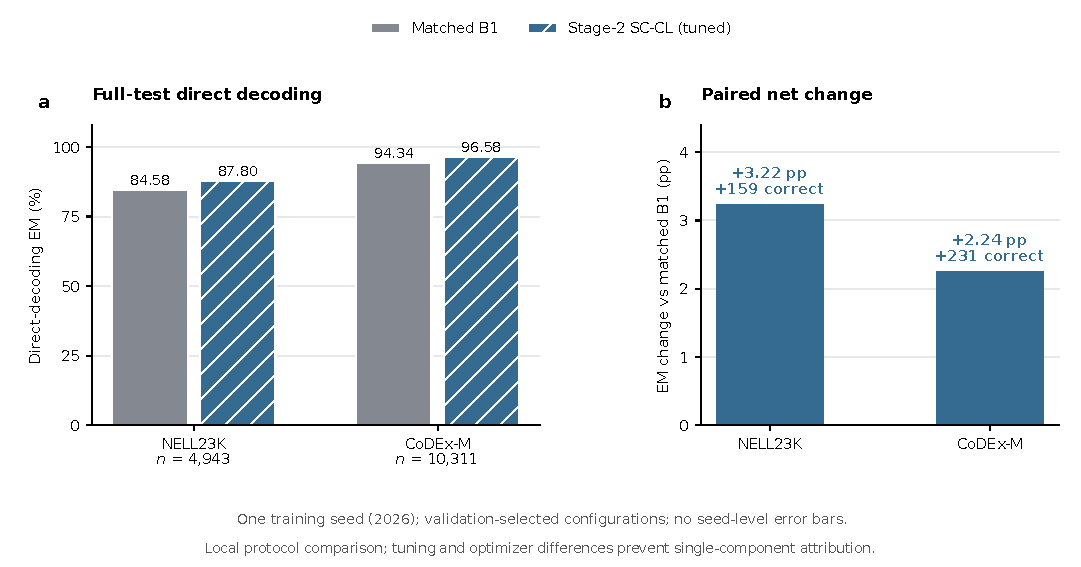
\includegraphics[width=\linewidth]{figures/python_results_20261103/fig01_direct_decoding.pdf}
  \caption{最新单种子本地协议的直接解码结果。a：匹配 B1 与验证选定的 Stage-2 SC-CL 配置在 NELL23K（4,943 题）和 CoDEx-M（10,311 题）的完整测试 EM。b：相对匹配 B1 的百分点差及净增正确题数。训练种子为 2026；无跨种子误差棒。结果涉及多项训练调参，不构成单一损失或采样信号的隔离收益。}
  \label{fig:python-latest-direct}
\end{figure}

\begin{figure}[tbp]
  \centering
  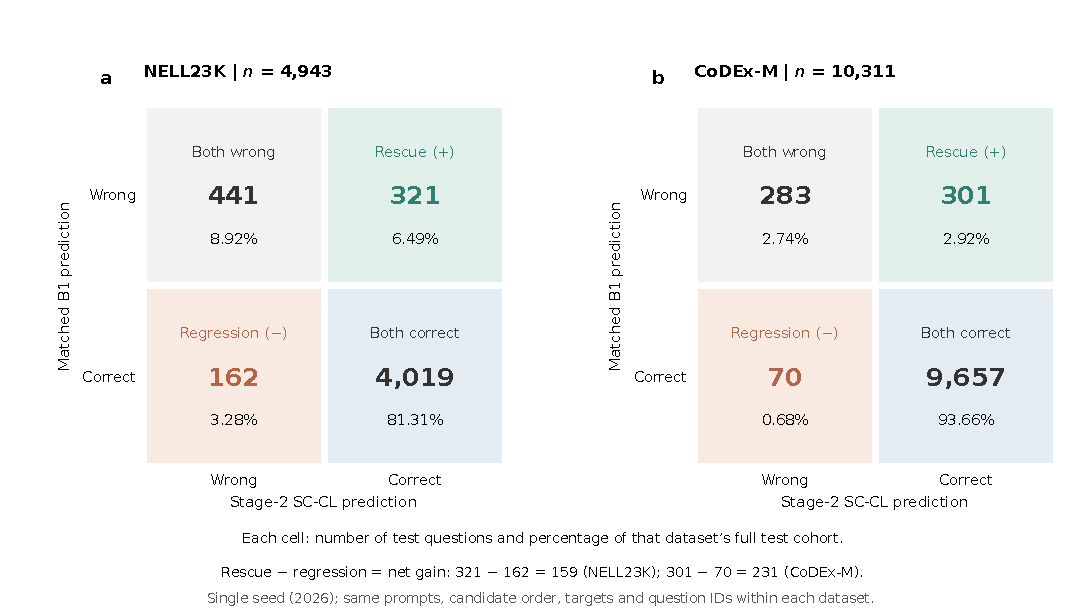
\includegraphics[width=\linewidth]{figures/python_results_20261103/fig02_paired_outcomes.pdf}
  \caption{最新直接解码的逐题配对变化。行为匹配 B1 的正确性，列为 Stage-2 SC-CL 的正确性，每格为题数及占该数据集全测试集的百分比。NELL23K 纠错 321 题、退化 162 题，净增 159；CoDEx-M 纠错 301 题、退化 70 题，净增 231。各数据集两模型的问题、候选顺序与目标一致，训练种子为 2026。}
  \label{fig:python-latest-paired}
\end{figure}

\begin{figure}[tbp]
  \centering
  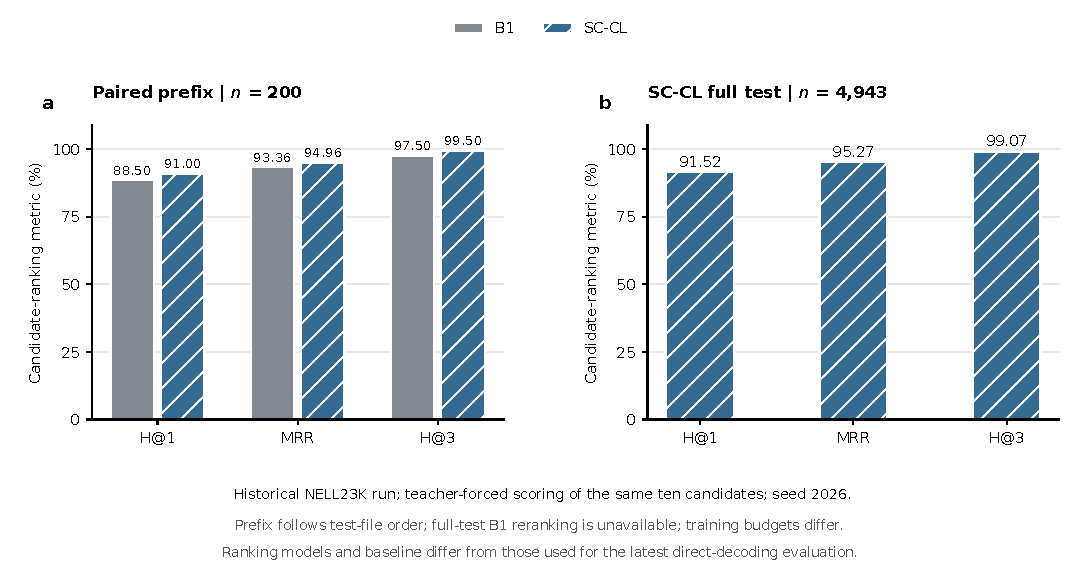
\includegraphics[width=\linewidth]{figures/python_results_20261103/fig03_historical_ranking.pdf}
  \caption{历史 NELL23K 模型的候选重排。a：测试文件前 200 题上相同十个候选的配对 H@1、MRR、H@3；b：SC-CL 全量 4,943 题排序指标。全量 B1 重排尚未完成，两模型训练预算不同。该历史排序模型及其基线与图~\ref{fig:python-latest-direct} 的最新直接解码模型不同，不能交叉推导收益。训练种子为 2026。}
  \label{fig:python-historical-ranking}
\end{figure}

\begin{table}[tbp]
  \caption{最新本地完整测试直接解码（训练种子 2026）。$\Delta$ 为相对匹配 B1 的百分点差。方法为验证选定的 Stage-2 SC-CL 配置；提示、候选顺序及答案配对，但训练调参尚未隔离。}
  \label{tab:python-latest-direct}
  \centering\small
  \begin{tabular}{lrrrrr}
    \toprule
    数据集 & $n$ & B1 EM（\%） & SC-CL EM（\%） & $\Delta$ & 净增题数 \\
    \midrule
    NELL23K & 4,943 & 84.58 & 87.80 & +3.22 & +159 \\
    CoDEx-M & 10,311 & 94.34 & 96.58 & +2.24 & +231 \\
    \bottomrule
  \end{tabular}
\end{table}
